\section{Evaluation and Results}
\label{sec:evaluation}
We evaluate Afar-prgenv against the functional readiness criteria defined in
Section~\ref{sec:metrics}. The emphasis is on correctness and compatibility
with PE libraries and MPI, which are prerequisites for any further performance
or application-level validation.

\begin{table}[t]
  \centering
  \small
  \setlength{\tabcolsep}{4pt}
  \caption{Repro suite coverage for the AFAR drop \afarversion. Status is
  recorded as P/S/F for each test.}
  \label{tab:repro}
  \begin{tabular}{l l c}
    \hline
    Test & Coverage & Status (P/S/F) \\
    \hline
    cmake-mpi-omp & CMake MPI+OMP & PASS \\
    compile-only & compiler sanity & PASS \\
    wrapper-compile-link & wrapper compile/link & PASS \\
    mpi-hello & MPI module integration & PASS \\
    omp-c & OpenMP offload (C) & PASS \\
    omp-f90 & OpenMP offload (F) & PASS \\
    libsci & PE math libs & PASS \\
    libsci-acc & accelerator libs & SKIP \\
    hdf5-parallel & HDF5 (par) & SKIP \\
    hdf5-serial & HDF5 (ser) & PASS \\
    fftw & FFTW (C/C++/F) & PASS \\
    dsmml & DSMML & PASS \\
    netcdf & PnetCDF & PASS \\
    \hline
  \end{tabular}
\end{table}

The `libsci-acc` profile is intentionally skipped; \texttt{libsci\_\allowbreak acc}
linking is not yet validated and may depend on ROCm 6 runtime libraries. The
parallel
HDF5 test is skipped due to missing HDF5 C++ `pkg-config` metadata, while the
serial HDF5 path passes.

\begin{figure}[t]
  \centering
  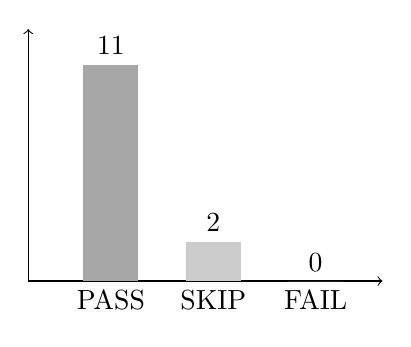
\begin{tikzpicture}[x=1cm, y=1cm]
  \def\barwidth{0.7}
  \def\scale{0.25}

  % Axes
  \draw[->] (0,0) -- (4.5,0);
  \draw[->] (0,0) -- (0,3.2);

  % PASS=11, SKIP=2, FAIL=0
  \fill[gray!70] (0.7,0) rectangle +( \barwidth, {11*\scale} );
  \fill[gray!40] (2.0,0) rectangle +( \barwidth, {2*\scale} );
  \fill[gray!20] (3.3,0) rectangle +( \barwidth, {0*\scale} );

  \node[below] at (1.05,0) {PASS};
  \node[below] at (2.35,0) {SKIP};
  \node[below] at (3.65,0) {FAIL};

  \node[above] at (1.05,{11*\scale}) {11};
  \node[above] at (2.35,{2*\scale}) {2};
  \node[above] at (3.65,0) {0};
\end{tikzpicture}

  \caption{Repro suite outcomes for \afarversion (unique tests).}
  \Description{Bar chart summarizing repro outcomes: 11 passes, 2 skips, 0 fails.}
  \label{fig:repro-summary}
\end{figure}

Across the repro matrix, 11 of 13 tests pass, 2 are skipped, and none fail.
Under our readiness policy, this qualifies the drop for extended validation
because the skips correspond to known external dependencies rather than
compiler regressions.

\begin{table}[t]
  \centering
  \small
  \setlength{\tabcolsep}{4pt}
  \caption{Skip causes observed in the \afarversion repro run.}
  \label{tab:skip-causes}
  \begin{tabular}{l p{0.62\columnwidth}}
    \hline
    Repro & SKIP cause \\
    \hline
    libsci-acc & ROCm 6 runtime dependencies missing for accelerator links. \\
    hdf5-parallel & Missing HDF5 C++ pkg-config metadata for the PE module. \\
    \hline
  \end{tabular}
\end{table}

\subsection{Compilation and Linking}
\label{sec:compile}
The repro matrix validates that AFAR drops compile and link with the PE
wrappers without requiring manual flag surgery. Wrapper diagnostics report any
filtered flags or mismatched MPI metadata early, which reduces support
turnaround when a drop regresses.
All workflow-focused repros (`compile-only`, `cmake-mpi-omp`, and
`wrapper-compile-link`) pass for \afarversion.
The CMake repro confirms that build systems can consume the wrappers without
manual flag translation.

\subsection{Repro Harness Coverage}
\label{sec:coverage}
The harness runs each profile under multiple module-order permutations, which
stress-test the wrapper logic that re-synchronizes `pkg-config` metadata at
compile time. This ensures that users can load library modules either before
or after `afar-prgenv` without breaking builds. In this evaluation, the base
profile and all library profiles completed without failures; the only
exceptions were the intentional skips noted in Table~\ref{tab:repro}.

\subsection{Module Ordering Robustness}
\label{sec:ordering}
To reflect real user behavior, we execute the repro suite across multiple
module load permutations (e.g., library modules loaded before or after
`afar-prgenv`). This checks that wrapper logic correctly re-synchronizes MPI
and library metadata regardless of module ordering. We report P/S/F outcomes
per permutation and flag any regressions for follow-up.

\begin{table}[t]
  \centering
  \small
  \setlength{\tabcolsep}{4pt}
  \caption{Module ordering permutations used to validate metadata
  re-synchronization.}
  \label{tab:ordering}
  \begin{tabular}{l l c}
    \hline
    Permutation & Example & Status (P/S/F) \\
    \hline
    Libs before AFAR & load libs, then afar-prgenv & PASS \\
    Libs after AFAR & load afar-prgenv, then libs & PASS \\
    MPI swap after AFAR & swap cray-mpich post-load & N/A \\
    \hline
  \end{tabular}
\end{table}

The before/after permutations pass for the library profiles exercised in this
study (LibSci, FFTW, DSMML, PnetCDF, and serial HDF5). MPI swap after AFAR is a
planned check and was not exercised in this run.

\subsection{MPI and Offload Validation}
\label{sec:mpi-offload}
MPI validation confirms that the wrappers resynchronize the MPI flavor on each
invocation, preventing stale `pkg-config` metadata when modules are swapped.
OpenMP offload tests confirm that `--offload-arch` is injected for both C and
Fortran workflows. This is exercised with the PE module
\texttt{craype-accel-}\allowbreak\texttt{amd-gfx90a}. Overrides via
\texttt{AFAR\_\*\_OFFLOAD\_ARCH} are also covered. The `mpi-hello`, `omp-c`, and
`omp-f90` repros all pass in this evaluation.

\subsection{Library Compatibility}
\label{sec:libraries}
Library repro tests confirm that AFAR drops can link against PE-provided HDF5,
FFTW, LibSci, DSMML, and PnetCDF libraries when the correct `pkg-config`
metadata is present. The `libsci-acc` path is treated as a conditional gate
because ROCm runtime dependencies can lag behind AFAR drops.
When the expected ROCm runtime libraries are present, `libsci-acc` builds
successfully; otherwise the test is skipped and the drop is held for follow-up.
The `libsci-acc` repro uses \texttt{AFAR\_LIBSCI\_ACC\_LIBNAME} to target the
correct accelerator library variant.

HDF5 validation uses an AFAR-compiled Fortran shim module to avoid incompatible
vendor \texttt{.mod} files while still linking against the HDF5 C libraries. The
PnetCDF repro relies on `pnetcdf.inc` instead of compiler-specific \texttt{.mod}
files, and it skips Fortran if the include file is absent. FFTW and DSMML
validation use `pkg-config` metadata and \texttt{scripts/check\_ldd.sh} to ensure the
link paths resolve to the expected PE libraries.

\subsection{Library Case Studies}
\label{sec:case-studies}
HDF5 highlights a common Fortran compatibility issue: vendor \texttt{.mod} files are
compiler-specific and often incompatible with AFAR. The repro uses an
AFAR-compiled shim module (\texttt{hdf5\_shim.f90}) so the Fortran build can
consume the PE-provided HDF5 C libraries without ingesting incompatible \texttt{.mod}
files. This pattern generalizes to other libraries that ship Fortran modules.

LibSci-acc highlights runtime dependency drift. Cray accelerator libraries may
link against ROCm 6 runtimes even when AFAR drops ship ROCm 7 toolchains. The
repro detects missing ROCm 6 libraries and reports a SKIP rather than a hard
FAIL, signaling a dependency gap rather than a compiler regression.

PnetCDF highlights module metadata gaps. The repro uses the Fortran include
\texttt{pnetcdf.}\allowbreak\texttt{inc} instead of compiler-specific module
files and skips Fortran validation when the include is missing. This keeps
the C/C++ checks active while isolating Fortran metadata gaps for follow-up.

\subsection{Binary Dependency Audits}
\label{sec:ldd}
Most repros run \texttt{scripts/check\_ldd.sh} after linking to verify that
library paths resolve to expected prefixes. The default allowlist includes PE
paths under \texttt{/opt/cray}, AFAR roots, and standard system locations
(e.g., \texttt{/lib*}, \texttt{/usr/lib*}), plus ROCm runtime paths required by
MPI. This audit catches accidental leakage to incompatible system libraries
and provides a fast signal for regressions introduced by a new drop.

\subsection{Metadata and Shim Coverage}
\label{sec:shims}
Shim \texttt{.pc} files are generated per profile when PE libraries do not expose
AFAR-compatible metadata. The wrappers append the shim directory to
\texttt{PKG\_CONFIG\_PATH} and optionally refresh it when the module
environment changes, which keeps library metadata stable even when users load
modules out of order. In practice, this is most important for Fortran-facing
libraries whose vendor `.pc` files omit module-specific include paths.

\subsection{Diagnostic Signals}
\label{sec:diagnostics-results}
The evaluation also tracks common failure signatures that indicate a drop is
not ready for broader validation. Examples include missing `pkg-config` data
for a loaded library module, a mismatch between \texttt{CRAY\_MPICH\_VERSION}
and the selected MPI flavor, and absent ROCm runtime dependencies for
accelerator libraries. The wrapper warnings and the repro harness logs capture
these cases early, enabling support teams to decide whether to regenerate
metadata, adjust module ordering, or defer the drop until dependencies align.

\begin{table}[t]
  \centering
  \small
  \setlength{\tabcolsep}{4pt}
  \caption{Common failure signals and mitigations.}
  \label{tab:failure-modes}
  \begin{tabular}{p{0.38\columnwidth} p{0.52\columnwidth}}
    \hline
    Signal & Mitigation \\
    \hline
    Missing `pkg-config` metadata & Regenerate shim `.pc` files and
    verify \texttt{PKG\_CONFIG\_PATH}. \\
    Wrong MPICH flavor selected & Rebuild via wrappers or reload
    \texttt{afar-prgenv} to resync \texttt{CRAY\_MPICH\_VERSION}. \\
    OpenMP offload arch missing & Load
    \texttt{craype-accel-}\allowbreak\texttt{amd-gfx90a} or set
    \texttt{AFAR\_FTN\_OFFLOAD\_ARCH}. \\
    LibSci-acc link fails & Check ROCm runtime deps or defer until matching
    accelerator libs are available. \\
    Incompatible Fortran \texttt{.mod} & Build AFAR-compatible shim modules. \\
    \hline
  \end{tabular}
\end{table}

\subsection{Operational Impact}
\label{sec:impact}
Operationally, Afar-prgenv converts AFAR drops from isolated toolchains into
PE-compatible environments. Support teams can validate a drop with a
deterministic repro suite and only escalate to broader validation (Fortran test
suites, OpenMP validation, and application builds) once the PE compatibility
baseline is satisfied.
In this run, the repro suite reported no failures; the only skips were
intentional gates for `libsci-acc` and the missing HDF5 C++ `pkg-config` data
in the parallel HDF5 path.

\subsection{Extended Validation}
\label{sec:extended-validation}
After repro gating, we run an OLCF Fortran application set and the SOLLVE
validation suite to evaluate readiness for production use. These suites provide
broader coverage of Fortran runtime behavior, OpenMP offload correctness, and
application build workflows that are not captured by the repro tests alone.

\begin{table}[t]
  \centering
  \caption{Extended validation suites used after repro gating.}
  \label{tab:extended}
  \begin{tabular}{l l l}
    \hline
    Suite & Coverage & Status (P/S/F) \\
    \hline
    OLCF Fortran apps & Fortran build/runtime & TBD \\
    SOLLVE V\&V & OpenMP offload & TBD \\
    \hline
  \end{tabular}
\end{table}
